\documentclass[11pt]{article}
\usepackage{graphicx}
\usepackage{hyperref}
\usepackage{caption}
\usepackage{amsmath}
\usepackage{color}
\usepackage{mathtools}
\usepackage{physics}
\usepackage{subcaption}
\newcommand{\numpy}{{\tt numpy}}    % tt font for numpy

\topmargin -.5in
\textheight 9in
\oddsidemargin -.25in
\evensidemargin -.25in
\textwidth 7in

\usepackage{dirtree}

\begin{document}

% ========== Edit your name here
\author{Hongqing Liu, hl85}
\title{CS 498: Assignment 5: 3D Multi Object Tracking}
\date{April 18, 2023}
\maketitle

\medskip


\section*{Submission}

In this assignment, you will code a 3D multi-object tracking system based on a Kalman filter. You will be submitting two files, ``kalman\_filter.py" and ``matching.py". Please put together a single PDF with your answers and figures for each problem, and submit it to Gradescope (Course Code: BBX6NE). 
We recommend you add your answers to the latex template files we provided. More details on what to report are in the provided code. 

\section*{Provided Files}

\textbf{Files you will modify}:
\begin{itemize}
    \item kalman\_filter.py: 
    \begin{itemize}
        \item define\_model (define dynamics)
        \item update (observation model)
        \item predict (state propagation)
    \end{itemize}
    \item matching.py (greedy matching algorithm)
    \item main.py (for visualization and debugging)
\end{itemize}

\noindent \textbf{Files you will not (need to) modify}:
\begin{itemize}
    \item evaluate.py: run this after running main.py to do evaluation, i.e. ``python evaluate.py"
    \item kitti\_calib/oxts.py: these are used for something called ego-motion-compensation, explained in code
    \item matching\_utils.py: contains the function iou(box\_a, box\_b) which you will need to compute similarity when doing matching
    \item utils.py: some utils used by main.py, you should look at Box3D
    \item vis.py: some code for visualizing the data. You only really need vis\_obj, which is described more clearly in main.py
\end{itemize}

File structure
\dirtree{%
.1 data.
.2 calib.
.3 training.
.4 [seq\_name].txt.
.2 detection.
.3 [seq\_name].txt.
.2 label.
.3 [seq\_name].txt.
.2 oxts.
.3 training.
.4 [seq\_name].txt.
.2 image\_02.
.3 training.
.4 [seq\_name].
.5 [frame\_num].png.
.1 results.
.2 eval (files in here will be created automatically).
.2 img\_vis (files in here will be created automatically).
}

\section*{Multi Object Tracking (MOT)} 

In this assignment, you will implement a multi object tracker for 3D objects. In other words, given a sequence of frames taken from the perspective of a car, track the other cars in the images. In this project we will develop our tracking algorithm on KITTI dataset(\url{http://www.cvlibs.net/datasets/kitti/}). 

The idea is as follows: we can use a good pre-trained object detector to find objects in each frame (we've already done that for you, check \url{https://github.com/sshaoshuai/PointRCNN} if you want to know more). Now, simply identifying objects is not good enough, so we want to track them across frames for consistency. You will implement two modules which together will do this quite well. 

The first is a matching algorithm: given a list of 3D bounding boxes for objects detected by the object detector in the current frame, match them to objects you are already tracking from the previous frame. 

The second is a Kalman Filter. Just matching current detections to past trackers is not great since cars can move and therefore the previous and current bounding boxes will not overlap perfectly (this is especially problematic if an object becomes occluded for a few frames). To deal with this issue you will implement a Kalman Filter for forward propagating each object. Moreover, you will now use each object detection to ``update" the state of your tracked object, as an observation to the filter.

\paragraph{Question 0 (Inspect the Data)[1 pt]:}
Before you begin the actual assignment, read the code we've provided. Namely read through ``main.py" so you understand the basic structure of the algorithm and the functionality of each component. You will need to modify ``main.py'' for debugging/visualization purposes. 

For this question, please visualize the detections for frame 100 of the first and second sequences, i.e. sequence 0000 and sequence 0001. Each detection should be a different color. You should work off the code we provided in the Visualization section of main.py.

Please download the images for the first sequence (0000), and put them in the right place in the directory structure above. Use your illinois address to access the drive link: \url{https://drive.google.com/file/d/15lWATvV4p9UCShnnPa2SEL8BTh2twIm4/view?usp=sharing}. This will allow you to overlay the sequence 0000 detections on top of the camera images for visualization. 

\textbf{Answers:} The result of visualization are shown as follows:

\begin{figure}[h]
    \centering
    \begin{subfigure}[b]{0.4\textwidth}
      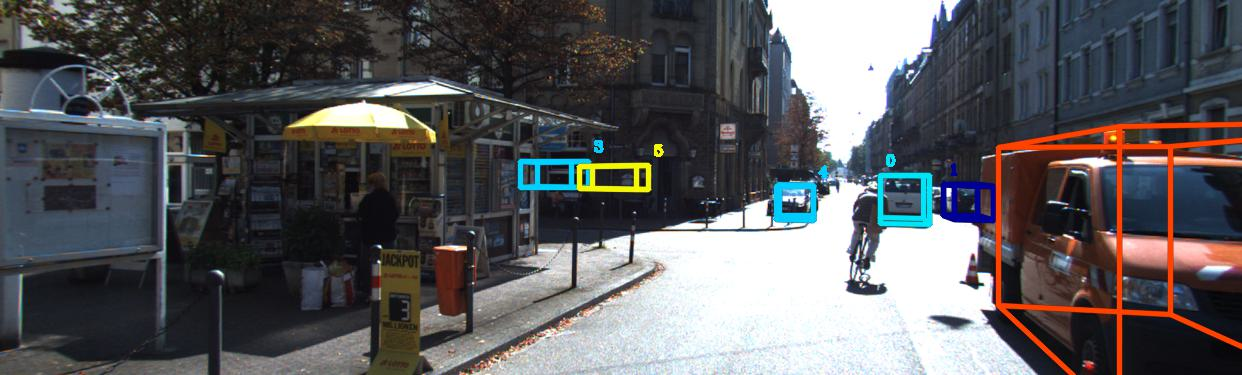
\includegraphics[width=\textwidth]{./fig/Q0_00_100.jpg}
      \caption{frame 100 in sequence 0000}
    \end{subfigure}
    \hfill
    \begin{subfigure}[b]{0.4\textwidth}
      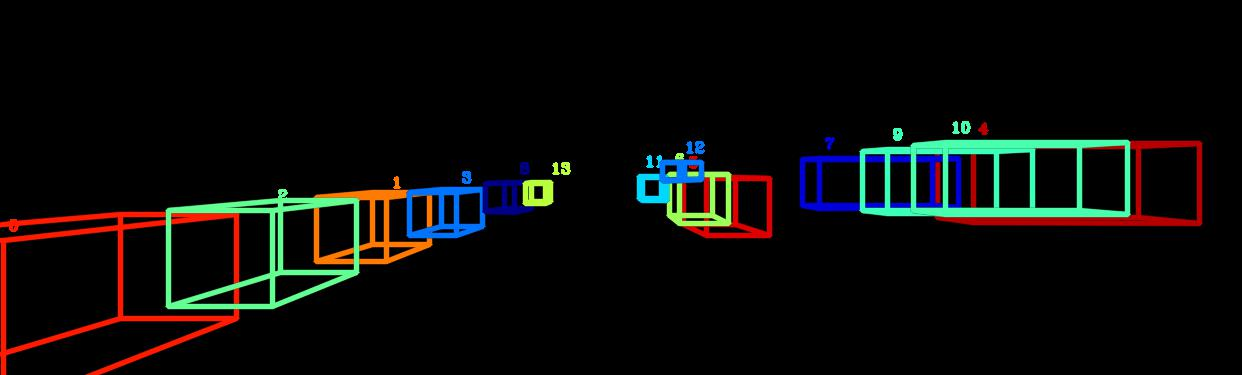
\includegraphics[width=\textwidth]{./fig/Q0_01_100.jpg}
      \caption{frame 100 in sequence 0001}
    \end{subfigure}
    % \caption{Two photos}
\end{figure}

\paragraph{Question 1 (Greedy Matching)[3 pt]:}
For this question you will be modifying ``matching.py". You should implement a greedy matching approach, whereby you match pairs of detections and tracked objects in order of similarity. First match the detection and tracker that are most similar, then remove them from the set, and continue, until you have no trackers or no detections. Also, if the similarity for a match is less than the provided threshold (-0.2), do not consider the pair a match.

Notice we provide you with ``iou(box\_a, box\_b)" to compute similarity (in terms of generalized IoU) between 3D detected regions.

\textbf{Answers:} The codes are shown as follows:

\begin{center}
    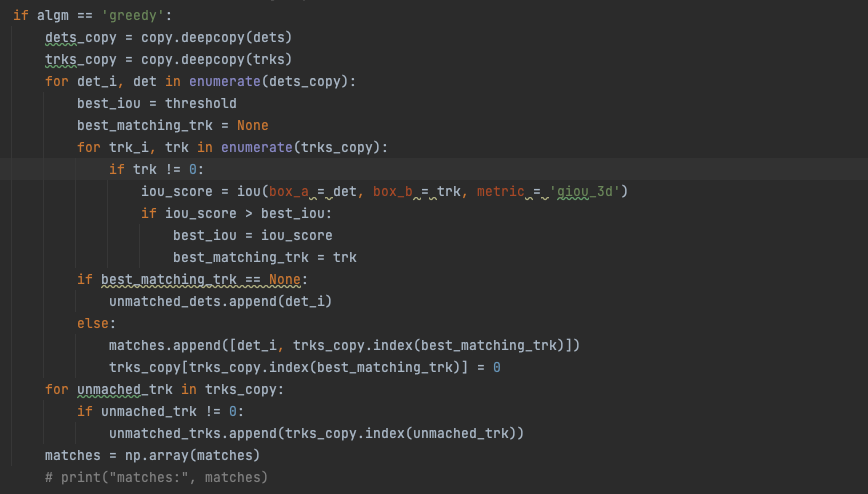
\includegraphics[width=0.3\textwidth]{./fig/Q1.png}
\end{center}

\paragraph{Question 2 (Trivial Update) [1 pt]:}
You'll notice that even though you've implemented matching, the trackers themselves don't update location. For this question you will implement a trivial update to each tracker in ``kalman\_filter.py". Given a matched detection z, simply set the associated tracker to have the same bounding box z. In other words, we simply trust the observation 100\% when updating the state, neglecting any motion or noise models.

In your pdf please show your code for this part, it should be very simple. Report your evaluation MOTA for this setting (meaning matching=greedy, predict() is unimplemented, and the update is trivial).

\textbf{Answers:} The codes and results are shown as follows, the MOTA is $0.7698$. The left image is codes for Trivial Update while the right image is the evaluation result.
\begin{center}
    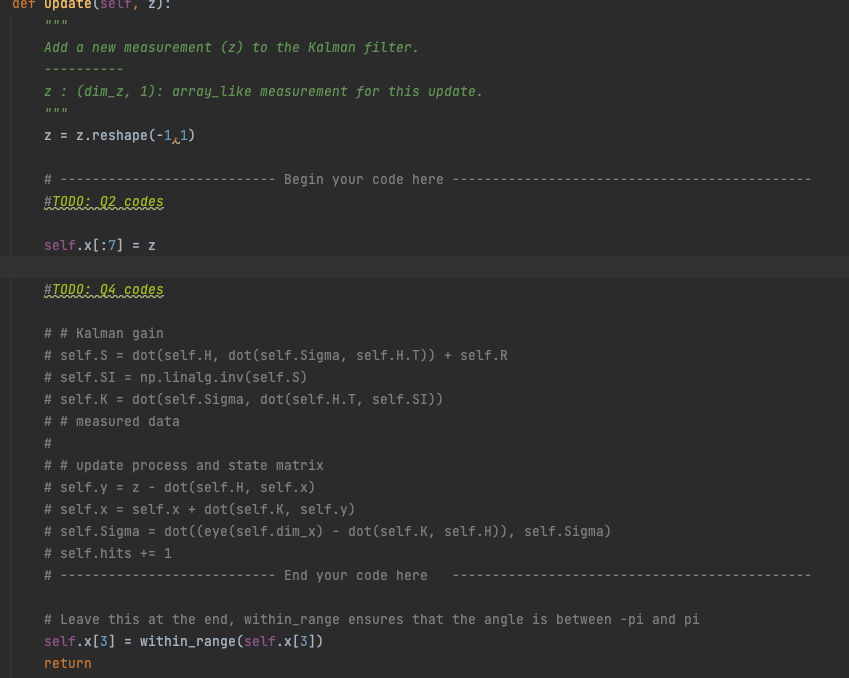
\includegraphics[width=0.3\textwidth]{./fig/Q2_code.png}
    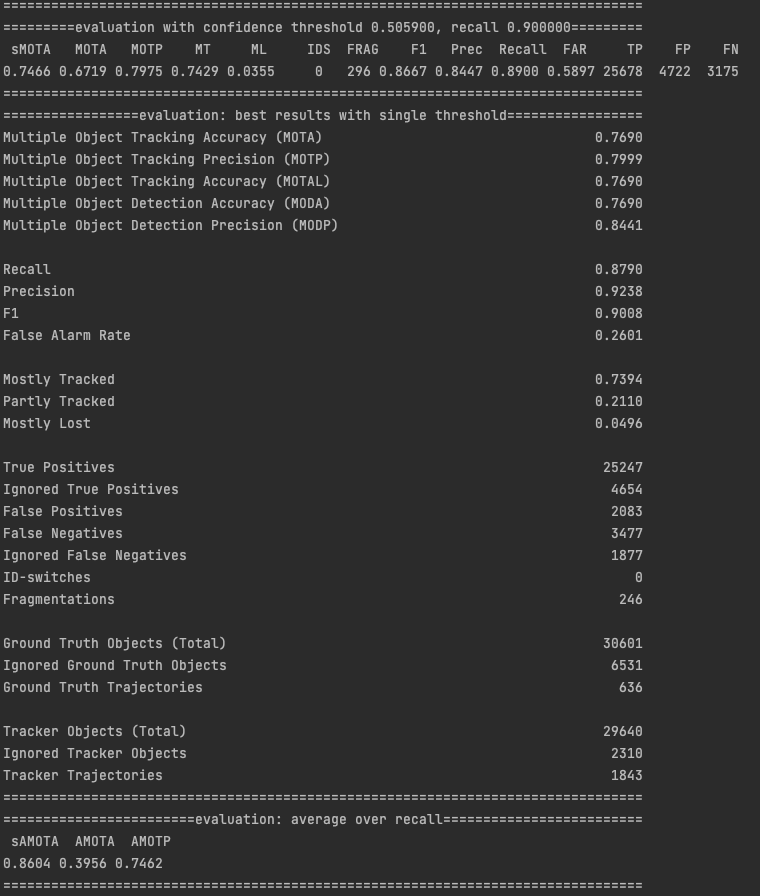
\includegraphics[width=0.3\textwidth]{./fig/Q2_result_all.png}
\end{center}

\paragraph{Question 3 (Kalman Linear Dynamics) [3 pt]:}
For this part you will fill in define\_model() in the class Kalman. The state $\mathbf{x}$ should consist three dimensional box center, raw angle, three dimensional box size, and finally three dimensional linear velocity (total 10D). The motion model is a constant linear velocity model in 3D. Your model should be linear, meaning x' = x + dx = Ax. In addition you should define the measurement model and measurement uncertainty, meaning H and Sigma and Q. In your pdf please report A, H, Sigma, Q, and R. Explain why each is set the way it is.

\textbf{Answers:} A is the transition matrix which represent the dynamic model for the state. The state x has $10$ dimensions: $x, y, z, theta, l, w, h, dx, dy, dz$
For the constant velocity model: 
\[x' = x + dx, \quad y' = y + dy, \quad z' = z + dz\]
while all others $theta, l, w, h, dx, dy, dz$ remain the same.
In tha case, the A is shown as follows:
\begin{center}
    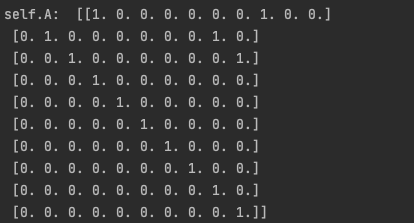
\includegraphics[width=0.3\textwidth]{./fig/Q3_A.png}
\end{center}

H is the measurement function, the first 7 dimensions of the measurement correspond to the state. The H is shown as follows:
\begin{center}
    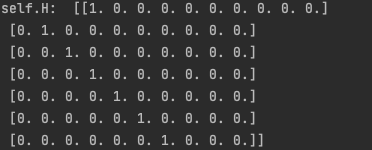
\includegraphics[width=0.3\textwidth]{./fig/Q3_H.png}
\end{center}

Sigma is the uncertainty vcovariance, Q is process uncertainty and R is measurement uncertinty, I tune them as follows to get a relatively good performance for multi object tracking
\begin{center}
    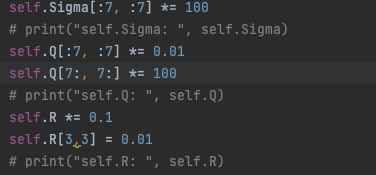
\includegraphics[width=0.3\textwidth]{./fig/Q3_para.png}
\end{center}

\paragraph{Question 4 (Kalman Update) [3 pt]:}
Now implement a proper Kalman Filter Update step, where you use a matched object detection as a noisy observation for updating the state (see lectures 11-12). 

In your pdf please describe the Kalman Filter linear update mathematically and report your evaluation MOTA under this setting (matching=greedy, predict() unimplemented, update implemented).

\textbf{Answers:} The update equations are shown as follows:
\begin{align}
    S_{t+1} &= H \Sigma_{t+1|t} H^T + R \label{eq:kf1}\\
    K_{t+1} &= \Sigma_{t+1|t} H^T S_{t+1}^{-1} \label{eq:kf2}\\
    \mu_{t+1} &= H \mu_{t+1|t} \label{eq:kf3}\\
    \mu_{t+1|t+1} &= \mu_{t+1|t} + K_{t+1} (z_{t+1} - \mu_{t+1}) \label{eq:kf4}\\
    \Sigma_{t+1|t+1} &= \Sigma_{t+1|t} - K_{t+1} H \Sigma_{t+1|t} \label{eq:kf5}
\end{align}
where $S_{t+1}$ is the innovation covariance, $K_{t+1}$ is the Kalman gain, $\Sigma_{t+1|t}$ is the predicted error covariance, $\mu_{z,t+1}$ is the predicted measurement, $\mu_{t+1|t}$ is the predicted state, $z_{t+1}$ is the actual measurement, $R$ is the measurement noise covariance, and $H$ is the measurement matrix. 

The evaluation result and codes are shown as follows, MOTA is 0.0791:
\begin{center}
    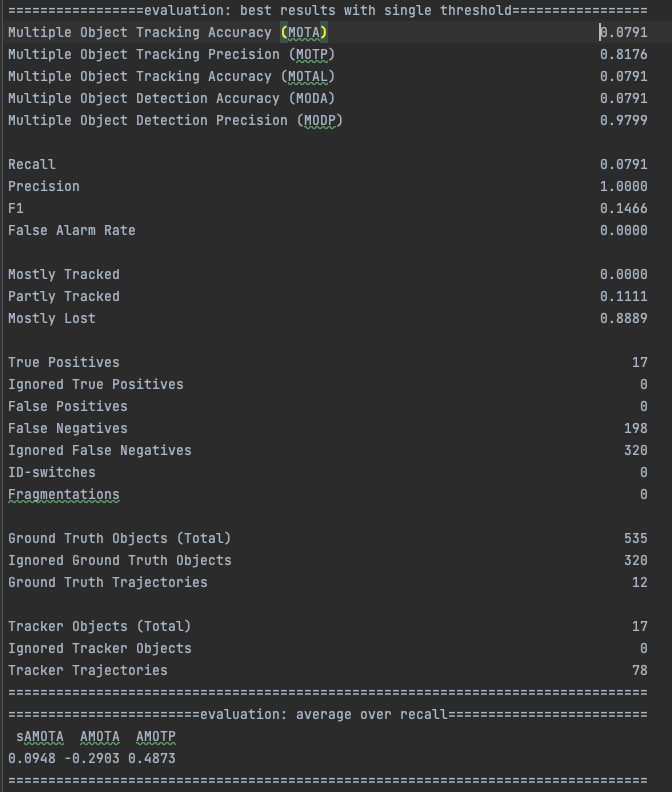
\includegraphics[width=0.3\textwidth]{./fig/Q4_result.png}
    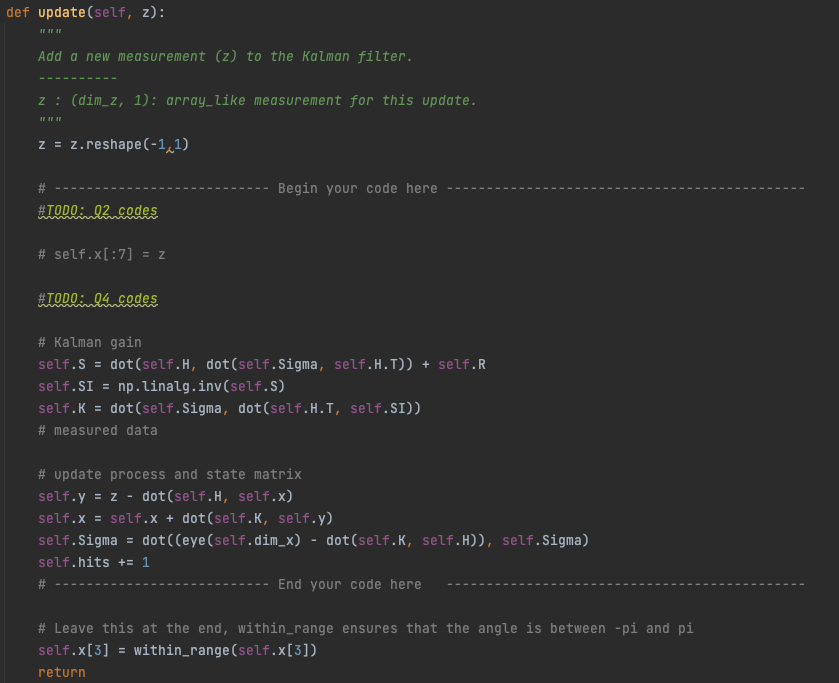
\includegraphics[width=0.3\textwidth]{./fig/Q4_code.png}
\end{center}

\paragraph{Question 5 (Kalman Predict) [2 pt]:}
Up until now, each frame the detections were compared to each tracker, and then matched trackers were updated. But our matching is poor because the detections and trackers do not overlap (they are one frame apart). In this question you will implement the Kalman Filter Predict step, where you forward propagate the state according to the dynamics model you defined earlier.

In your pdf please describe the predict step, and report your evaluation MOTA under this setting (matching=greedy, predict and update both implemented).

\textbf{Answers:} The predict function is shown as follows:
\begin{align}
    \mu_{t+1|t} &= A\mu_{t|t} + B\underline{u}_{t} \label{eq:kf6}\\
    \Sigma_{t+1|t} &= A\Sigma_{t|t}A^T + GQG^T \label{eq:kf7}
\end{align}

The evaluation result and codes are shown as follows, MOTA is 0.7701:
\begin{center}
    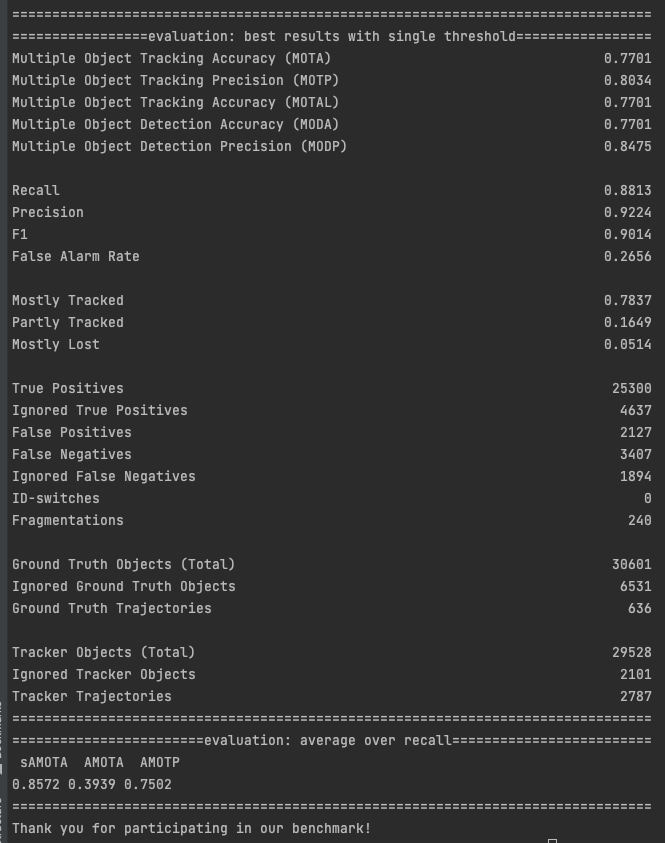
\includegraphics[width=0.3\textwidth]{./fig/Q5_results.png}
    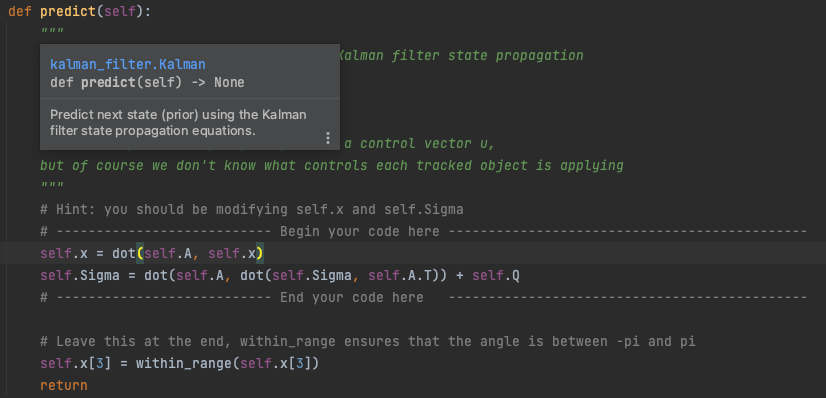
\includegraphics[width=0.3\textwidth]{./fig/Q5_code.png}
\end{center}

\paragraph{Question 6 (Final Visualization) [1 pt]:}
Please visualize some results from your final code. 
Pick at least 4 consecutive frames from sequence 0000. For each frame visualize all in one image:
\begin{itemize}
    \item Show birthed trackers in green
    \item Show dead trackers in red
    \item For the rest of the trackers (these were matched), show each before and after update. Show their corresponding detections as well. Color the trackers in blue and detections in yellow. Add text above each tracker with its ID and the text ``-" for before update or ``+" for after update.  
\end{itemize}

\textbf{Answers:} As shown in the follows BOX9 appears at frame 5 and track as visualized after update in frame 6 and disappear at frame 9. Meanwhile, BOX0 is tracking steady in the whole process.

\begin{figure}[h]
    \centering
    \begin{subfigure}[b]{0.4\textwidth}
      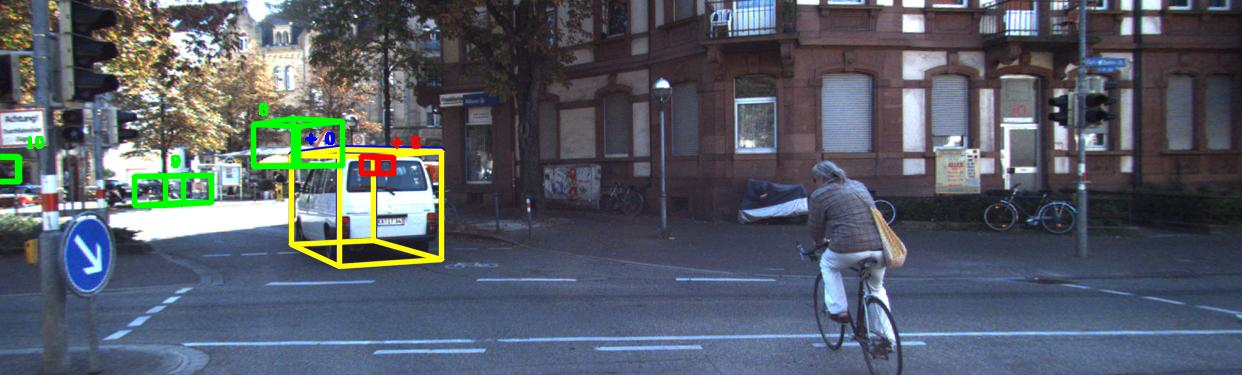
\includegraphics[width=\textwidth]{./fig/Q6_5.jpg}
      \caption{frame 5 in sequence 0000}
    \end{subfigure}
    \hfill
    \begin{subfigure}[b]{0.4\textwidth}
        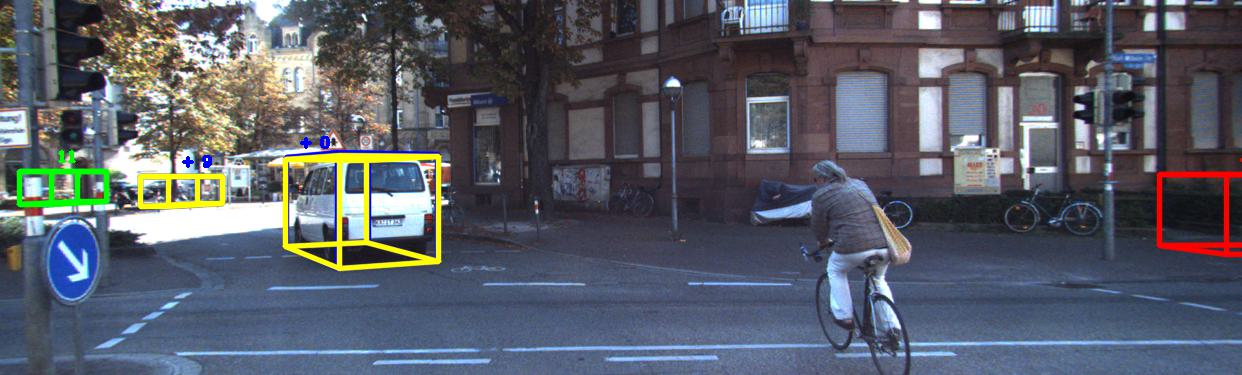
\includegraphics[width=\textwidth]{./fig/Q6_6.jpg}
        \caption{frame 6 in sequence 0000}
    \end{subfigure}
    \hfill
    \begin{subfigure}[b]{0.4\textwidth}
        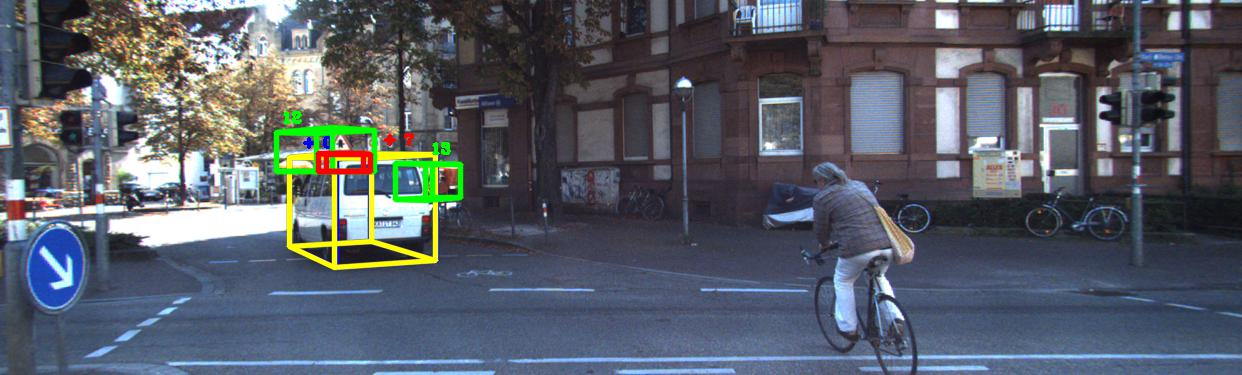
\includegraphics[width=\textwidth]{./fig/Q6_7.jpg}
        \caption{frame 7 in sequence 0000}
    \end{subfigure}
    \hfill
    \begin{subfigure}[b]{0.4\textwidth}
        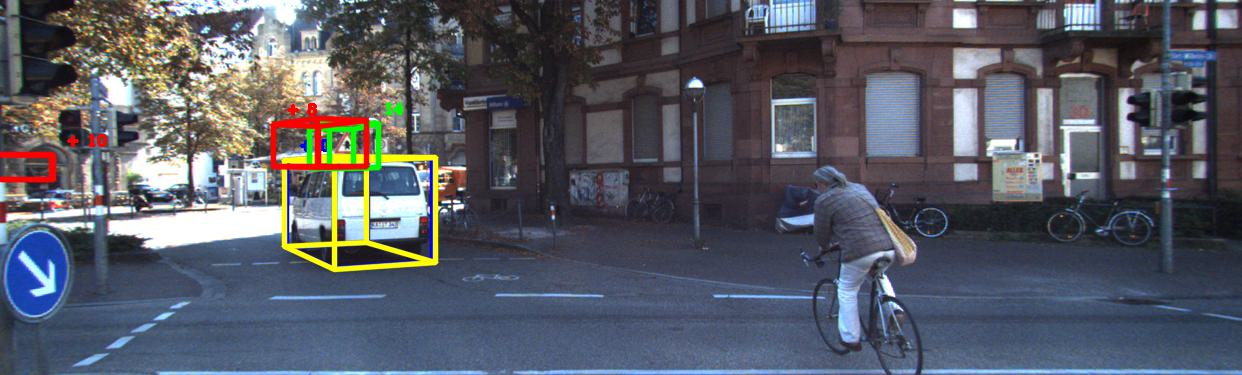
\includegraphics[width=\textwidth]{./fig/Q6_8.jpg}
        \caption{frame 8 in sequence 0000}
    \end{subfigure}
    \hfill
    \begin{subfigure}[b]{0.4\textwidth}
        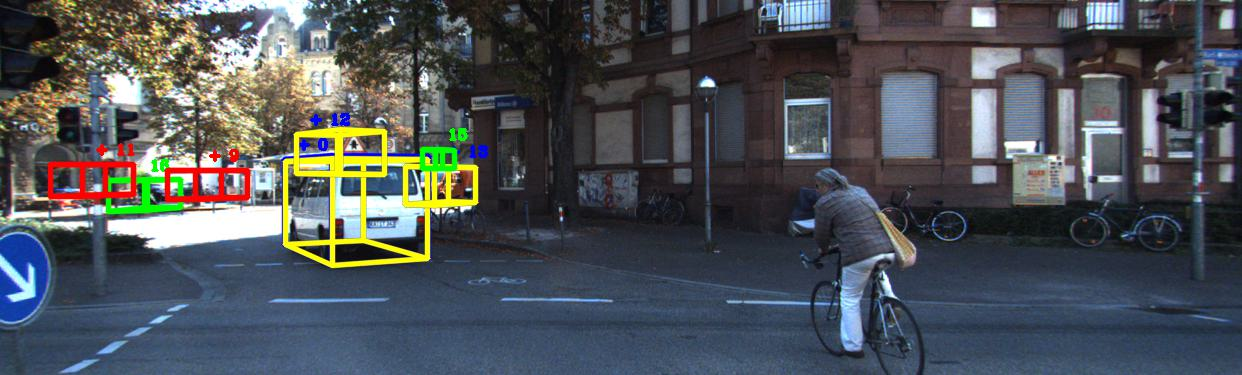
\includegraphics[width=\textwidth]{./fig/Q6_9.jpg}
        \caption{frame 9 in sequence 0000}
    \end{subfigure}
    \hfill
    \begin{subfigure}[b]{0.4\textwidth}
        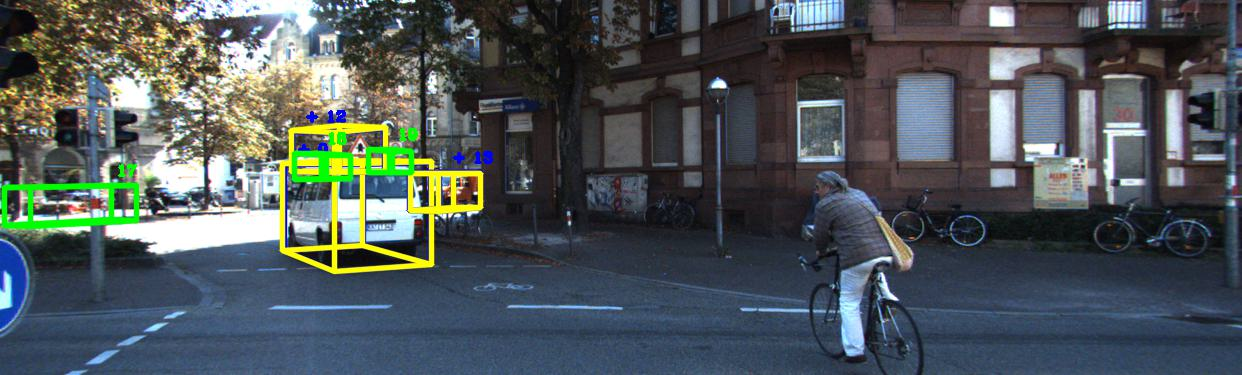
\includegraphics[width=\textwidth]{./fig/Q6_10.jpg}
        \caption{frame 10 in sequence 0000}
    \end{subfigure}
    % \caption{Two photos}
\end{figure}

\paragraph{Question 7 (Analysis) [1 pt]:}
Please run the run \texttt{python evaluate.py} and report your MOTA, TPs, ID switches, FRAGs and FPs at the best threshold. Please also visualize at least two failure cases and explain the reason. Please discuss what can be done to avoid these failures.  

\textbf{Answers:} MOTA: 0.7701, TPs: 25300, ID switches: 0, FRAGs: 240, FPs 2127, the best threshold is -0.2.

\begin{center}
    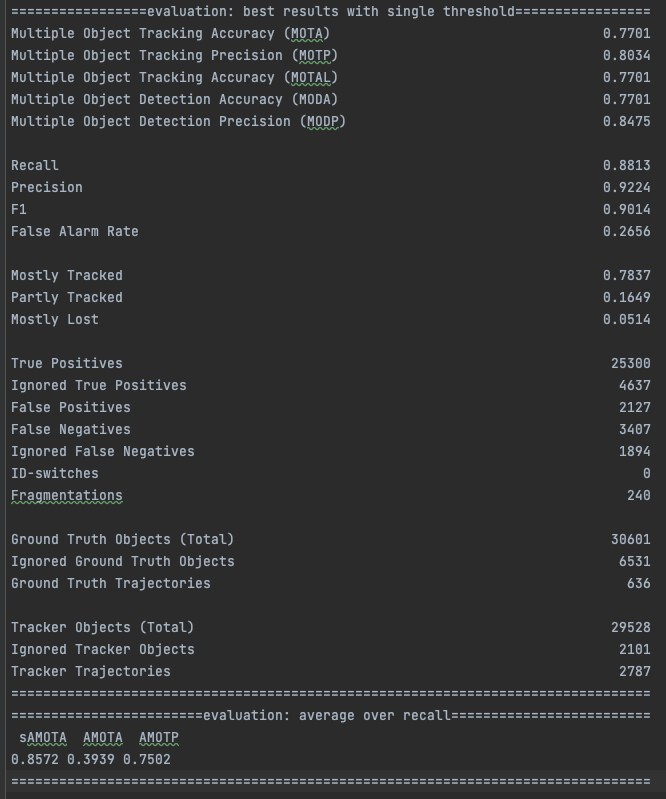
\includegraphics[width=0.7\textwidth]{./fig/Q7_result.png}
\end{center}

Failure case 1: The detector detects too many bounding boxes that are not targets. This will increase the computational complexity of the system.

Like what I showed below in frame 9 in sequence 0000, there are too many detections in the frame which are not the traget, this is caused by the detectio error of detector network model. If the model is overfitted, we can use more training data or use regularization techniques to prevent it.

\begin{center}
    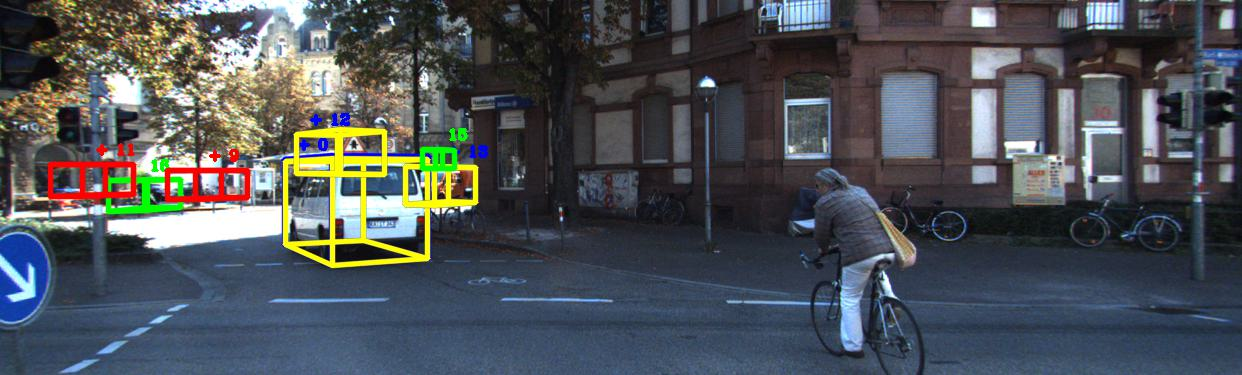
\includegraphics[width=0.7\textwidth]{./fig/Q6_9.jpg}
\end{center}

Failure case 2: When the tracking object is blocked by other item, the tracking box disappear. This will caused the discontinuity of tracking.

Like what I showed below in frame 82 in sequence 0000, the tracker of the white car(box 0) disappears after white car is blocking. To solve this problem, we can add a estimator for object blocking by other object. this estimator is built based on the motion model of the tracking target.

\begin{center}
    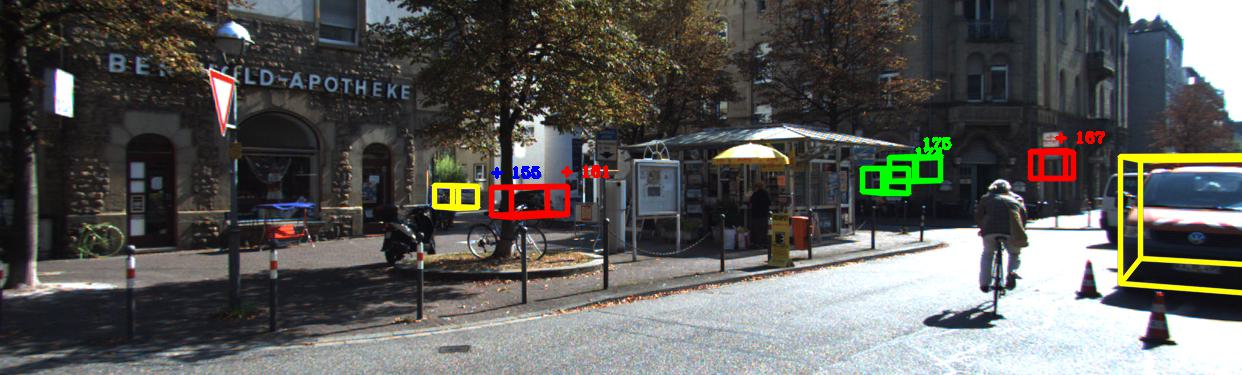
\includegraphics[width=0.7\textwidth]{./fig/Q7_82.jpg}
\end{center}

\paragraph{Bonus Question (Option 1: Better Matching) [3 pt Bonus]:}
Improve your matching algorithm from greedy to the Hungarian algorithm. You must implement it yourself. Alternatively improve your matching by training a neural network to perform matching based on more than just spatial proximity. Report the tracking performance and compare it against the IOU-based greedy matching through both qualitative and quantitative results. Do you see a performance improvement? Discuss the comparison study results.

\paragraph{Bonus Question (Option 2: Better Dynamics) [3 pt Bonus]:}
Make your Kalman filter into an extended Kalman filter and implement a bicycle model for dynamics instead of linear. \url{https://www.coursera.org/lecture/intro-self-driving-cars/lesson-2-the-kinematic-bicycle-model-Bi8yE}. 
Report the tracking performance and compare it against linear velocity model through both qualitative and quantitative results. Do you see a performance improvement?  Discuss the comparison study results.

\end{document}. 

\grid
\grid